\chapter{Solution}
\label{solution}



\begin{enumerate}
\item Create a Sample (see on kliendile, testiks ja prototüübiks)
\item Develop the course Materials (peab teadma activities + tagasiside review)
\item Conduct a Run-through (real-time rehearsal testi sõbra peal kogu kursust +  feedback assessment + saab reaalselt teada aja, mis kulub kursuse läbimisele
\end{enumerate}


The implementation phase of the ADDIE Model contains three sub-phases

\begin{enumerate}
\item Train the Instructor
\item Prepare the Learners
\item Arrange the Learning Space
\end{enumerate}

Train the Instructor - course developer is often a trainer too but some cases you need more people to train


Development:
Authoring
Media creation / integration / production
Prototyping
Processing
Quality Assurance

\section{Development of the e-learning course}

\subsection{Authoring the learning material}
In the development phase the authoring of learning materials, tests, media and integration of all artefacts into consistent body. 

\url{http://www.grayharriman.com/ADDIE.htm}

\begin{table}[h]
\centering
\caption{The learning materials}

\begin{tabular}{|p{5cm}|p{3cm}|p{6cm}|}
\hline 
\color{blue}
Name & \color{blue} Comments  & \color{blue} Location \\ 

\hline
  \multicolumn{3}{|c|}{Pre-requirement course} \\
\hline
Operating system basics & & \\
\hline
Basic networking IPv4/IPv6, TCP/IP & & \\

\hline
GNU/Linux basics (and OpenBSD/FreeBSD basics)  & & \\
\hline
Scripting in BASH &  & \\
\hline
Scripting in Python & Co authored with Lauri Võsandi & \\
\hline
Scripting in PowerShell & Author is Heiki Tähis & \\


\hline
\hline
  \multicolumn{3}{|c|}{Root services} \\

\hline 


Lecture - Configuring NTP service & (Estonian 2012), Learning outcome no XXX & \url{http://goo.gl/toRpw} \\ 
\hline 
Practical class - Configuring NTP in Ubuntu  & (Estonian 2012), Learning outcome no XXX , Students improved & \url{https://wiki.itcollege.ee/index.php/NTP_Ubuntus} \\
\hline 
Lecture DNS & & \href{http://enos.itcollege.ee/~mernits/infrastruktuur/Interneti%20domeeninimede%20s%c3%bcsteem%20-%20IT%20infra%20loeng.odp}
{DNS Lecture [OpenDocument]} \\
\hline
Practical class - DNS & Co authored with Katrin Loodus  & \href{https://docs.google.com/document/d/1ZeQpPXdVq1C7RQpxQYR0gBB0OBMYB_0g6aFFxs_-fIA/edit}{Configuring DNS [GoogleDocs] } \\

\hline
\hline
  \multicolumn{3}{|c|}{Web/File Services} \\

\hline 
 & & \\
\hline

\hline
 & & \\
\hline
\hline
  \multicolumn{3}{|c|}{E-mail service} \\
\hline 
 & & \\
\hline

\hline
 & & \\

\hline
\hline
  \multicolumn{3}{|c|}{IP firewalls and IDS/IPS} \\
\hline 
 & & \\
\hline

\hline
 & & \\

\hline
\hline
  \multicolumn{3}{|c|}{Autentication and authorization} \\
\hline 
 & & \\
\hline

\hline
 & & \\

\hline
 & & \\
\hline
\end{tabular} 
\label{table:learning_materials}
\end{table}


\subsection{Text based learning material}
Developed learning material should follow consistent style and present also one example of good documentation practice. For system administrators several howto styles exists. However practical hands-on laboratory instructions are designed that pass through using copy paste is possible but gives one working sample. However, this is not enough to pass lab scenario and student must customize own configuration.

Guiding stile of the lab instruction using style convention: First, all variable parts of the text are clearly differs from other text and command. Second, all commands given by student are highlighted, and variable parts embossed as seen in followed command.


\begin{minted}[frame=lines,framesep=2mm]{bash}
#Sample for changing OOM adjustment score for mysql server
echo "-17" > /proc/$(pidof mysqld)/oom_adj
\end{minted}
%$


Sample sample: Finding a proccess ID of the mysql server proccess.

\begin{minted}[frame=lines,framesep=2mm]{bash}
ps -ef|grep mysqld
\end{minted}
\label{code_sample}
%
\small{
\begin{Verbatim}[frame=single,
label=Command output,framesep=2mm,rulecolor=\color{red},commandchars=\\\{\}]
sudent@opiise:~# ps -ef|grep mysqld
root     11290 10905  0 10:27 pts/6    00:00:00 grep --color=auto mysqld
mysql    \fbox{\color{red}29830}    1  0 Apr25 ?        00:05:47 /usr/sbin/mysqld
\end{Verbatim}
%
}

All study should stored in open formats, like pdf, OpenDocument , MediaWiki markup language, html, utf8 text. Original editable source files for generating pdf, images should be publicly accessible. Moreover, text based materials should stored into version control system like git or subversion to enable contributing for other lecturers and students as well.

\subsection{Audio/Visual learning material}
The Audio/Visual material is recorded from live lectures and practical classes using echo360 equipment or screen/audio recording for some classes. Recordings are supportive materials and not the main source for knowledge.

\url{http://echo360.e-uni.ee/ess/portal/section/36936084-4fbb-413c-98ec-0470f11db4e3}


\subsection{Interactive learning material}

\subsection{Online tests and laboratory scenarios}

\subsection{Learning objectives}

\subsection{Technical implementation of the e-course}

\LaTeX Minted muutujad jne


\subsubsection{The Environment of Distance Study}
\label{The Environment of Distance Study}
The Environment of Distance Study...

TODO pilt virtuaalaborite süsteemi kontekstist
\subsubsection{Random tags}
\begin{itemize}
	\item normal traffic generator
	\item malicious traffic generator
	\item availability monitor (for grading)
\end{itemize}

\subsubsection{Virtualization Layer}
Siin libvirdist
\subsubsection{Web Application Layer}
Siin Ruby on Rails raamistikust ja veebirakendusest
\subsubsection{Architecture of Distance Laboratory}
Siin räägin üldisest disainist ja allsüsteemidest
\
\begin{figure}[ht]
\centering
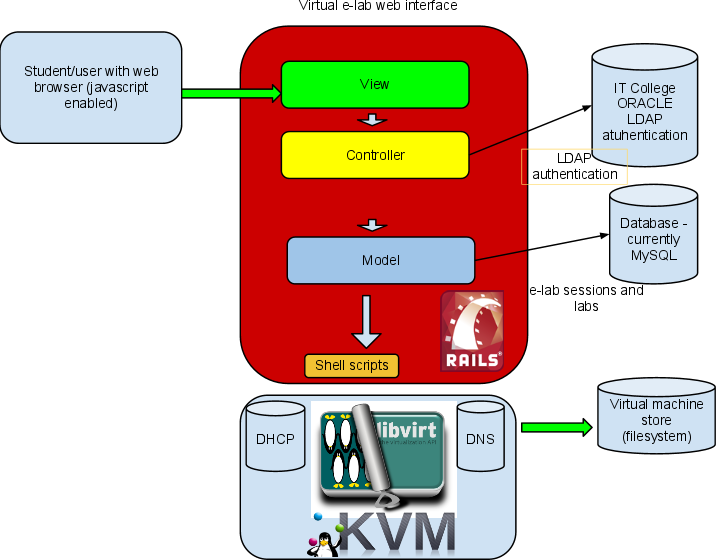
\includegraphics[width=0.8\textwidth]{architecture.png}
\caption{Architecture of Distance Laboratory}
\label{fig:Architecture of Distance Laboratory}
\end{figure}
\

\subsubsection{Security Aspects of Distance Laboratory}

\subsection{Testing the e-course}

\section{Piloting the course}

\subsection{Organizational role}

\subsection{Social role}

\subsection{Pedagogical role}